\chapter{SYSTEM DESIGN AND PROTOCOL ARCHITECTURE}

\section{ARCHITECTURAL OVERVIEW}
The core innovation of the Hybrid Post-Quantum Voice (\textbf{HPQV}) protocol is the strict architectural decoupling of control-plane security establishment from data-plane real-time media transport. Rather than attempting to force multi-kilobyte post-quantum cryptographic primitives into an unreliable datagram substrate, HPQV divides the communication lifecycle across two parallel, specialized transport channels:

\begin{figure}[htbp]
    \centering
    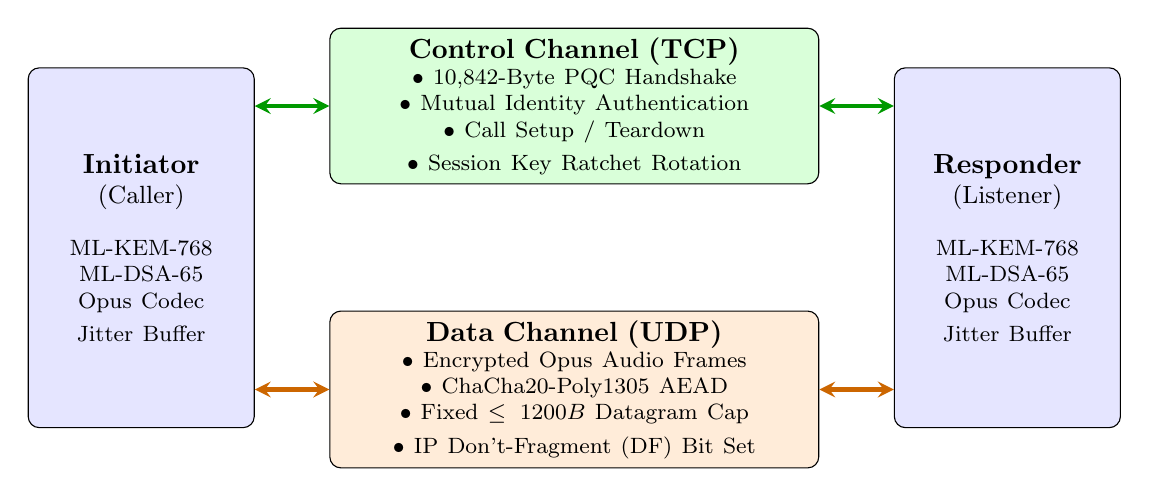
\begin{tikzpicture}[
        every node/.style={align=center},
        peer/.style={rectangle, draw, fill=blue!10, text width=7.5em, align=center, rounded corners, minimum height=13em},
        channel_tcp/.style={rectangle, draw, fill=green!15, text width=17em, align=center, minimum height=4.5em, rounded corners},
        channel_udp/.style={rectangle, draw, fill=orange!15, text width=17em, align=center, minimum height=4.5em, rounded corners},
        link/.style={thick, <->, >=stealth}
    ]
        \node [peer] (init) at (-5.5, 0) {\textbf{Initiator}\\\small (Caller)\\[1em]\footnotesize ML-KEM-768\\ML-DSA-65\\Opus Codec\\Jitter Buffer};
        \node [channel_tcp] (tcp) at (0, 1.8) {\textbf{Control Channel (TCP)}\\\footnotesize $\bullet$ 10,842-Byte PQC Handshake\\$\bullet$ Mutual Identity Authentication\\$\bullet$ Call Setup / Teardown\\$\bullet$ Session Key Ratchet Rotation};
        \node [channel_udp] (udp) at (0, -1.8) {\textbf{Data Channel (UDP)}\\\footnotesize $\bullet$ Encrypted Opus Audio Frames\\$\bullet$ ChaCha20-Poly1305 AEAD\\$\bullet$ Fixed $\le 1200\text{ B}$ Datagram Cap\\$\bullet$ IP Don't-Fragment (DF) Bit Set};
        \node [peer] (resp) at (5.5, 0) {\textbf{Responder}\\\small (Listener)\\[1em]\footnotesize ML-KEM-768\\ML-DSA-65\\Opus Codec\\Jitter Buffer};

        \draw [link, color=green!60!black, line width=1.5pt] (init.east |- tcp.west) -- (tcp.west);
        \draw [link, color=green!60!black, line width=1.5pt] (tcp.east) -- (resp.west |- tcp.east);
        
        \draw [link, color=orange!80!black, line width=1.5pt] (init.east |- udp.west) -- (udp.west);
        \draw [link, color=orange!80!black, line width=1.5pt] (udp.east) -- (resp.west |- udp.east);
    \end{tikzpicture}
    \caption{HPQV Decoupled Dual-Channel Transport Architecture.}
    \label{fig:hpqv_architecture}
\end{figure}

As depicted in Figure \ref{fig:hpqv_architecture}, the two communicating endpoints establish two concurrent connections:
\begin{enumerate}
    \item \textbf{Control Channel (TCP):} A reliable, connection-oriented byte stream that carries the post-quantum cryptographic key exchange, mutual identity verification, signaling messages (\texttt{CALL\_START}, \texttt{CALL\_END}), and forward-secret key ratchet rotations. Because TCP provides transparent byte-stream segmentation and guaranteed delivery via sliding-window retransmissions, the 10,842-byte post-quantum handshake never becomes an IP fragment.
    \item \textbf{Data Channel (UDP):} An unreliable, connectionless datagram path dedicated solely to streaming encrypted Opus voice frames. Datagrams are strictly constrained under a conservative 1,200-byte cap and transmitted with the IPv4 Don't-Fragment (DF) flag asserted. The data plane maintains near-zero queueing latency, delegating frame loss recovery to in-band forward error correction and jitter buffering.
\end{enumerate}

\section{CONTROL CHANNEL SPECIFICATION (TCP)}

\subsection{Framing and Record Layer}
Because TCP is an unformatted byte stream lacking native record boundaries, the HPQV control layer introduces an application-level length-prefixed framing protocol. Every discrete control and cryptographic record transmitted over TCP is encapsulated within a 4-byte big-endian header indicating the payload length:
\begin{equation}
    \text{Record} = \text{Length}\ (4\ \text{bytes, unsigned big-endian integer}) \parallel \text{Payload}\ (L\ \text{bytes})
\end{equation}
The receiver's socket driver executes a bounded reassembly loop (\texttt{\_recvn}), blocking until exactly $L$ bytes have been extracted from the OS kernel buffer. This framing guarantees that variable-length post-quantum messages are parsed unambiguously without risk of TCP stream boundary fragmentation.

\subsection{Control Message Protocol}
Post-handshake session signaling utilizes structured control messages prefixed with a 1-byte message type identifier:
\begin{table}[htbp]
    \centering
    \caption{HPQV Control Plane Message Definitions.}
    \label{tab:control_messages}
    \begin{tabularx}{\textwidth}{>{\raggedright\arraybackslash}p{4.2cm} c >{\raggedright\arraybackslash}p{2.5cm} >{\raggedright\arraybackslash}X}
        \toprule
        \textbf{Identifier} & \textbf{Type Value} & \textbf{Payload} & \textbf{Operational Semantics} \\
        \midrule
        \texttt{MSG\_CALL\_START} & \texttt{0x01} & UDP Port (2B) & Signals readiness to stream voice; exchanges remote UDP port. \\
        \texttt{MSG\_CALL\_END} & \texttt{0x02} & None & Initiates graceful call termination and teardown. \\
        \texttt{MSG\_KEY\_ROTATE} & \texttt{0x03} & None & Instructs peers to ratchet the symmetric session key in lockstep. \\
        \bottomrule
    \end{tabularx}
\end{table}

\section{CRYPTOGRAPHIC HANDSHAKE DESIGN}

\subsection{Cryptographic Primitives and Parameter Selection}
HPQV deploys NIST Security Category 3 lattice-based primitives:
\begin{itemize}
    \item \textbf{Key Encapsulation Mechanism:} ML-KEM-768 \cite{nist_fips203}, operating on rank $k=3$ module lattices over $R_q = \mathbb{Z}_{3329}[X]/(X^{256}+1)$, offering 192 bits of classical security and robust resistance against quantum search algorithms.
    \item \textbf{Digital Signature Algorithm:} ML-DSA-65 \cite{nist_fips204}, parameterized over module lattices with matrix dimensions $(k,\ell) = (6,5)$ and modulus $q=8380417$.
\end{itemize}

\subsection{Handshake Message Structure}
The cryptographic handshake consists of a 2-message exchange: \texttt{HELLO} and \texttt{ACCEPT}.

\subsubsection{1. Initiator HELLO (6,445 Bytes)}
The caller initiates communication by generating an ephemeral ML-KEM-768 keypair $(\text{pk}_{\text{KEM}}, \text{sk}_{\text{KEM}})$. It concatenates this public key with its long-term ML-DSA-65 identity public key $\text{pk}_{\text{DSA}}^{\text{init}}$ and computes a digital signature over both keys using its private identity key $\text{sk}_{\text{DSA}}^{\text{init}}$:
\begin{equation}
    \sigma_{\text{init}} = \text{Sign}_{\text{ML-DSA-65}}(\text{sk}_{\text{DSA}}^{\text{init}}, \text{pk}_{\text{KEM}} \parallel \text{pk}_{\text{DSA}}^{\text{init}})
\end{equation}
The formatted \texttt{HELLO} message wire layout is:
\begin{equation}
    \text{HELLO} = \text{Version}\ (1\text{B}) \parallel \text{pk}_{\text{KEM}}\ (1184\text{B}) \parallel \text{pk}_{\text{DSA}}^{\text{init}}\ (1952\text{B}) \parallel \sigma_{\text{init}}\ (3309\text{B})
\end{equation}
Total byte length $= 1 + 1184 + 1952 + 3309 = \mathbf{6,445\ \text{bytes}}$.

\subsubsection{2. Responder ACCEPT (4,397 Bytes)}
Upon receiving \texttt{HELLO}, the responder extracts the public keys and verifies the initiator's identity against its pinned trust store. If valid, the responder encapsulates a 256-bit shared secret using $\text{pk}_{\text{KEM}}$:
\begin{equation}
    (\text{ct}_{\text{KEM}}, K_{\text{shared}}) = \text{Encap}_{\text{ML-KEM-768}}(\text{pk}_{\text{KEM}})
\end{equation}
The responder authenticates the exchange by computing its own ML-DSA-65 signature over the transcript:
\begin{equation}
    \sigma_{\text{resp}} = \text{Sign}_{\text{ML-DSA-65}}(\text{sk}_{\text{DSA}}^{\text{resp}}, \text{pk}_{\text{KEM}} \parallel \text{ct}_{\text{KEM}})
\end{equation}
The formatted \texttt{ACCEPT} wire layout is:
\begin{equation}
    \text{ACCEPT} = \text{Version}\ (1\text{B}) \parallel \text{ct}_{\text{KEM}}\ (1088\text{B}) \parallel \sigma_{\text{resp}}\ (3309\text{B})
\end{equation}
Total byte length $= 1 + 1088 + 3309 = \mathbf{4,397\ \text{bytes}}$. Combined handshake total is $\mathbf{10,842\ \text{bytes}}$.

\begin{figure}[htbp]
    \centering
    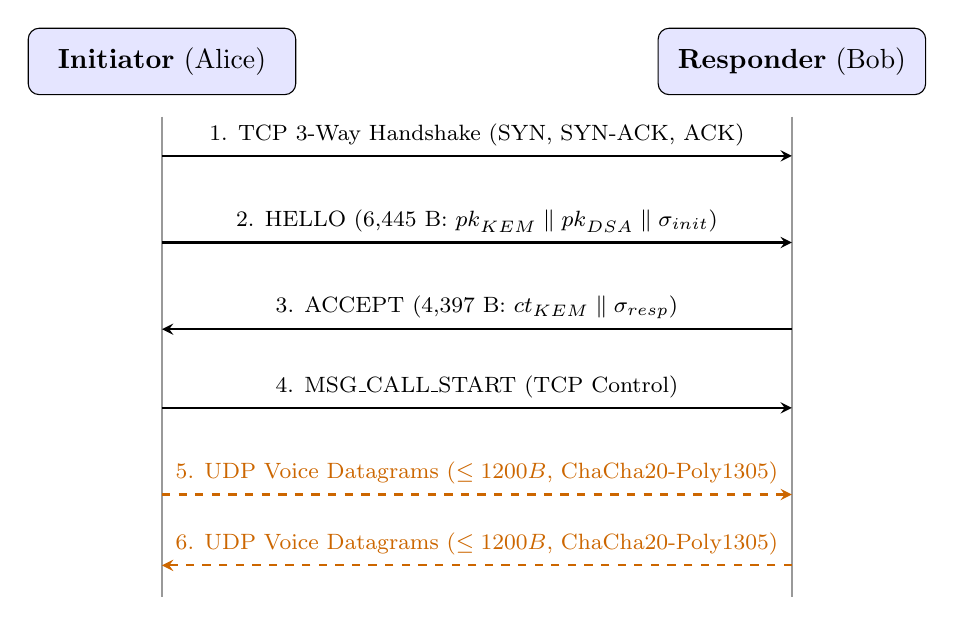
\begin{tikzpicture}[
        every node/.style={align=center},
        entity/.style={rectangle, draw, fill=blue!10, text width=9em, align=center, minimum height=2.4em, rounded corners},
        msg/.style={thick, ->, >=stealth},
        mediamattr/.style={thick, ->, >=stealth, dashed, color=orange!80!black}
    ]
        \node [entity] (init) at (-4, 5.0) {\textbf{Initiator} (Alice)};
        \node [entity] (resp) at (4, 5.0) {\textbf{Responder} (Bob)};
        
        \draw [thick, black!40] (-4, 4.3) -- (-4, -1.8);
        \draw [thick, black!40] (4, 4.3) -- (4, -1.8);

        \draw [msg] (-4, 3.8) -- node[above]{\footnotesize 1. TCP 3-Way Handshake (SYN, SYN-ACK, ACK)} (4, 3.8);
        \draw [msg] (-4, 2.7) -- node[above]{\footnotesize 2. HELLO (6,445 B: $\text{pk}_{\text{KEM}} \parallel \text{pk}_{\text{DSA}} \parallel \sigma_{\text{init}}$)} (4, 2.7);
        \draw [msg] (4, 1.6) -- node[above]{\footnotesize 3. ACCEPT (4,397 B: $\text{ct}_{\text{KEM}} \parallel \sigma_{\text{resp}}$)} (-4, 1.6);
        \draw [msg] (-4, 0.6) -- node[above]{\footnotesize 4. MSG\_CALL\_START (TCP Control)} (4, 0.6);
        
        \draw [mediamattr] (-4, -0.5) -- node[above]{\footnotesize 5. UDP Voice Datagrams ($\le 1200\text{ B}$, ChaCha20-Poly1305)} (4, -0.5);
        \draw [mediamattr] (4, -1.4) -- node[above]{\footnotesize 6. UDP Voice Datagrams ($\le 1200\text{ B}$, ChaCha20-Poly1305)} (-4, -1.4);
    \end{tikzpicture}
    \caption{Sequential Execution Flow of the HPQV Protocol.}
    \label{fig:handshake_sequence}
\end{figure}

\section{MUTUAL AUTHENTICATION AND TRANSCRIPT BINDING}

\subsection{Vulnerability Analysis of Unilateral Authentication}
During initial development, the handshake prototype implemented unilateral authentication: while the initiator authenticated its identity via $\sigma_{\text{init}}$, the responder's \texttt{ACCEPT} message contained only the raw ciphertext $\text{ct}_{\text{KEM}}$.

As documented in Architecture Decision Record 0002 (ADR-0002), this unilateral design possessed a severe Man-in-the-Middle (MITM) vulnerability. An active network adversary $\mathcal{A}$ on the TCP control path could observe the unauthenticated \texttt{ACCEPT} message, discard it, and substitute its own encapsulated ciphertext $\text{ct}'_{\mathcal{A}}$ derived from the initiator's public $\text{pk}_{\text{KEM}}$. Because the initiator lacked cryptographic proof that the ciphertext originated from the intended peer, it would decapsulate $\text{ct}'_{\mathcal{A}}$, establishing a shared key with the adversary rather than the legitimate responder.

\subsection{Cryptographic Transcript Binding (ADR-0002)}
To eliminate MITM attacks, HPQV mandates mutual authentication. The responder must possess an out-of-band pinned identity key $\text{pk}_{\text{DSA}}^{\text{resp}}$. In the \texttt{ACCEPT} record, the responder binds the cryptographic transcript by signing the exact concatenation of the initiator's public key and the resulting ciphertext:
\begin{equation}
    \mathcal{M}_{\text{transcript}} = \text{pk}_{\text{KEM}} \parallel \text{ct}_{\text{KEM}}
\end{equation}
Prior to executing decapsulation, the initiator verifies $\sigma_{\text{resp}}$ against the trusted $\text{pk}_{\text{DSA}}^{\text{resp}}$:
\begin{equation}
    \text{Verify}_{\text{ML-DSA-65}}(\text{pk}_{\text{DSA}}^{\text{resp}}, \mathcal{M}_{\text{transcript}}, \sigma_{\text{resp}}) \stackrel{?}{=} \text{True}
\end{equation}
If verification fails, the connection aborts immediately with an \texttt{unpinned identity} or \texttt{bad signature} exception. This transcript binding guarantees that an adversary cannot alter or substitute the encapsulation.

\section{KEY DERIVATION AND DIRECTIONAL NONCE SEPARATION}

\subsection{HKDF Expansion}
Following successful decapsulation, both peers possess an identical 256-bit post-quantum shared secret $K_{\text{shared}}$. HPQV expands this secret using the HMAC-based Key Derivation Function (HKDF-SHA256, RFC 5869) \cite{rfc5869}:
\begin{equation}
    \text{OKM} = \text{HKDF-Expand}(\text{PRK} = K_{\text{shared}}, \text{info} = \text{b"hpqv v1"}, \text{length} = 40)
\end{equation}
The 40-byte output keying material ($\text{OKM}$) is sliced into three distinct cryptographic values:
\begin{equation}
    K_{\text{voice}} = \text{OKM}[0:32],\quad \text{Prefix}_{I \to R} = \text{OKM}[32:36],\quad \text{Prefix}_{R \to I} = \text{OKM}[36:40]
\end{equation}
\begin{itemize}
    \item $K_{\text{voice}}$: A 256-bit symmetric key dedicated to data-plane ChaCha20-Poly1305 encryption.
    \item $\text{Prefix}_{I \to R}$: A 4-byte nonce prefix for voice packets traveling from Initiator to Responder.
    \item $\text{Prefix}_{R \to I}$: A 4-byte nonce prefix for voice packets traveling from Responder to Initiator.
\end{itemize}

\subsection{Elimination of Nonce Reuse Vulnerabilities}
The construction of distinct directional nonce prefixes solves a critical cryptographic hazard. ChaCha20-Poly1305 (RFC 7539) is an Authenticated Encryption with Associated Data (AEAD) cipher requiring a 96-bit (12-byte) nonce \cite{rfc7539}. It is a well-established cryptographic fact that reusing a single (Key, Nonce) pair under ChaCha20-Poly1305 completely destroys authenticity: an adversary observing two ciphertexts encrypted under identical nonces can XOR the ciphertexts to recover plaintext differences and compute the underlying Poly1305 authenticator key, permitting undetected ciphertext forgery.

In a full-duplex VoIP session, both endpoints begin streaming audio simultaneously, each initializing their sequence counter at zero ($\text{seq} = 0$). If both directions utilized a shared nonce prefix, the initiator's first packet and the responder's first packet would possess identical 12-byte nonces:
\begin{equation}
    \text{Nonce}_{I \to R}(0) = \text{Prefix} \parallel 0 = \text{Nonce}_{R \to I}(0)
\end{equation}
By deriving two mathematically independent 4-byte prefixes from HKDF and enforcing:
\begin{align}
    \text{Nonce}_{I \to R}(\text{seq}) &= \text{Prefix}_{I \to R}\ (4\text{B}) \parallel \text{seq}\ (8\text{B, big-endian}) \\
    \text{Nonce}_{R \to I}(\text{seq}) &= \text{Prefix}_{R \to I}\ (4\text{B}) \parallel \text{seq}\ (8\text{B, big-endian})
\end{align}
HPQV strictly partitions the nonce spaces, ensuring that identical nonces are never generated across the lifetime of the session.

\section{DYNAMIC KEY ROTATION AND RATCHETING}
To maintain forward secrecy throughout long-duration calls, HPQV implements an HKDF-based key ratchet mechanism. Either endpoint can trigger key rotation by dispatching an authenticated \texttt{MSG\_KEY\_ROTATE} control record over TCP.

Both endpoints ratchet their symmetric state deterministically:
\begin{equation}
    \text{OKM}_{\text{next}} = \text{HKDF-Expand}(\text{PRK} = K_{\text{current}}, \text{info} = \text{b"hpqv rotate v1"}, \text{length} = 40)
\end{equation}
Extracting:
\begin{equation}
    K_{\text{new}} = \text{OKM}_{\text{next}}[0:32],\quad P_0 = \text{OKM}_{\text{next}}[32:36],\quad P_1 = \text{OKM}_{\text{next}}[36:40]
\end{equation}
To ensure that peers maintain mirrored send and receive prefix assignments without ambiguity, prefixes are mapped via a canonical lexicographic comparison:
\begin{equation}
    (\text{SendPrefix}_{\text{new}}, \text{RecvPrefix}_{\text{new}}) = 
    \begin{cases}
        (P_0, P_1), & \text{if } \text{SendPrefix}_{\text{current}} < \text{RecvPrefix}_{\text{current}} \\
        (P_1, P_0), & \text{otherwise}
    \end{cases}
\end{equation}
Upon ratcheting, packet sequence numbers reset to zero ($\text{seq} = 0$), and the old session key is overwritten in memory.

\section{DATA CHANNEL SPECIFICATION (UDP)}

\subsection{Voice Datagram Header and AEAD Framing}
The HPQV voice datagram layout is engineered for minimal framing overhead while providing complete packet authenticity:

\begin{figure}[htbp]
    \centering
    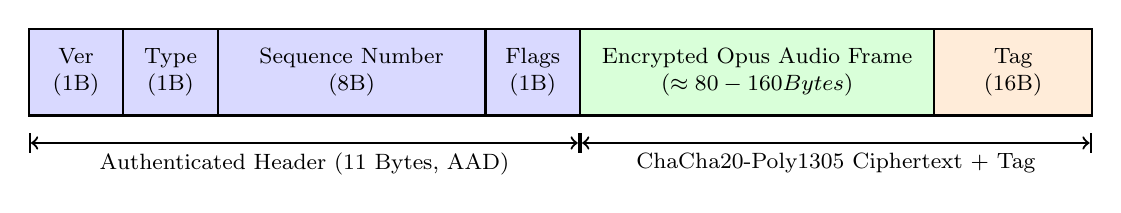
\begin{tikzpicture}[
        every node/.style={align=center, font=\footnotesize}
    ]
        \draw[thick, fill=blue!15] (0,0) rectangle (1.2,1.1) node[pos=.5]{Ver\\(1B)};
        \draw[thick, fill=blue!15] (1.2,0) rectangle (2.4,1.1) node[pos=.5]{Type\\(1B)};
        \draw[thick, fill=blue!15] (2.4,0) rectangle (5.8,1.1) node[pos=.5]{Sequence Number\\(8B)};
        \draw[thick, fill=blue!15] (5.8,0) rectangle (7.0,1.1) node[pos=.5]{Flags\\(1B)};
        \draw[thick, fill=green!15] (7.0,0) rectangle (11.5,1.1) node[pos=.5]{Encrypted Opus Audio Frame\\($\approx 80-160\text{ Bytes}$)};
        \draw[thick, fill=orange!15] (11.5,0) rectangle (13.5,1.1) node[pos=.5]{Tag\\(16B)};

        % Dimension lines below boxes
        \draw[thick, |<->|] (0,-0.35) -- (7.0,-0.35) node[midway, below]{Authenticated Header (11 Bytes, AAD)};
        \draw[thick, |<->|] (7.0,-0.35) -- (13.5,-0.35) node[midway, below]{ChaCha20-Poly1305 Ciphertext + Tag};
    \end{tikzpicture}
    \caption{HPQV Data-Plane Voice Datagram Layout.}
    \label{fig:packet_layout}
\end{figure}

As shown in Figure \ref{fig:packet_layout}, the unencrypted header occupies exactly 11 bytes:
\begin{equation}
    \text{Header} = \text{Ver}\ (1\text{B}) \parallel \text{Type}\ (1\text{B}) \parallel \text{SeqNum}\ (8\text{B}) \parallel \text{Flags}\ (1\text{B})
\end{equation}
This 11-byte header is supplied as Associated Authenticated Data (AAD) to the ChaCha20-Poly1305 cipher. Any tampering with sequence numbers, packet types, or flags causes decryption to fail.

\subsection{Enforced Datagram Invariant and DF Flag}
To ensure that data-plane traffic never experiences IP-layer fragmentation under any network condition, HPQV implements a dual-layer architectural invariant:
\begin{enumerate}
    \item \textbf{Application-Level Sizing Guard:} The datagram serialization function (\texttt{packet.seal}) explicitly evaluates the assembled packet size. If the length exceeds 1,200 bytes, the function raises an immediate runtime exception:
    \begin{equation}
        \text{Length}(\text{Header} \parallel \text{Ciphertext} \parallel \text{Tag}) \le 1200\ \text{bytes}
    \end{equation}
    Because standard 20 ms Opus frames compress speech to 80--160 bytes, the total datagram size typically spans 110--190 bytes—well below the 1,200-byte threshold.
    \item \textbf{Kernel-Level Don't-Fragment Bit:} The underlying UDP socket is initialized with explicit operating system socket options setting the Don't-Fragment (DF) flag (\texttt{IP\_MTU\_DISCOVER} with \texttt{IP\_PMTUDISC\_DO} on Linux; \texttt{IP\_DONTFRAGMENT} on Windows). If an anomalous packet exceeds path MTU, the OS drops the packet locally rather than fragmenting it.
\end{enumerate}

\section{AUDIO PROCESSING AND RESILIENCE PIPELINE}

\subsection{Opus Codec Integration}
HPQV processes wideband audio at 48,000 Hz (48 kHz) mono with 16-bit linear PCM. Audio frames are grouped into 20 ms chunks:
\begin{equation}
    \text{Frame Samples} = 48000 \times 0.020 = 960\ \text{samples} = 1,920\ \text{bytes PCM}
\end{equation}
The Opus encoder operates in \texttt{APPLICATION\_VOIP} mode with in-band Forward Error Correction (LBRR) active.

\subsection{Jitter Buffer Architecture}
Network packet arrival over UDP is non-deterministic. To resolve packet reordering, delay jitter, and duplicate deliveries, HPQV incorporates a fixed-depth min-heap jitter buffer (depth $D=3$ frames, corresponding to 60 ms buffer depth).
\begin{algorithm}[htbp]
\caption{HPQV Jitter Buffer Ingestion and Extraction}
\label{alg:jitter_buffer}
\begin{algorithmic}[1]
\Require Sequence number $s$, Audio payload $f$, State: $\text{Heap } H$, $\text{SeenSet } S$, $\text{LastSeq } L$, Depth $D$
\Procedure{Push}{$s, f$}
    \If{$s \le L$ \textbf{or} $s \in S$}
        \State \Return \Comment{Discard duplicate or stale packet}
    \EndIf
    \State $S \gets S \cup \{s\}$
    \State $\text{HeapPush}(H, (s, f))$
\EndProcedure
\Procedure{Pop}{}
    \If{$\text{Length}(H) < D$}
        \State \Return $\text{None}$ \Comment{Buffering to absorb network jitter}
    \EndIf
    \State $(s_{\text{min}}, f_{\text{min}}) \gets \text{HeapPop}(H)$
    \State $S \gets S \setminus \{s_{\text{min}}\}$
    \State $L \gets s_{\text{min}}$
    \State \Return $f_{\text{min}}$
\EndProcedure
\end{algorithmic}
\end{algorithm}
As detailed in Algorithm \ref{alg:jitter_buffer}, incoming frames are inserted into min-heap $H$. Packets with sequence numbers older than the last popped packet ($s \le L$) are dropped as expired. Only when buffer occupancy reaches depth $D$ does \texttt{Pop()} extract the lowest sequence number, ensuring perfectly ordered playout.
